% Created 2015-06-08 lun. 08:37
\documentclass[11pt,xcolor=dvipsnames,presentation]{beamer}
\usepackage[utf8]{inputenc}
\usepackage[T1]{fontenc}
\usepackage{fixltx2e}
\usepackage{graphicx}
\usepackage{longtable}
\usepackage{float}
\usepackage{wrapfig}
\usepackage{rotating}
\usepackage[normalem]{ulem}
\usepackage{amsmath}
\usepackage{textcomp}
\usepackage{marvosym}
\usepackage{wasysym}
\usepackage{amssymb}
\usepackage{hyperref}
\tolerance=1000
\usedescriptionitemofwidthas{bl}
\usepackage[T1]{fontenc}
\usepackage[utf8]{inputenc}
\usepackage[american, english]{babel}
\usepackage{ifthen,figlatex,amsmath,amstext,gensymb,amssymb}
\usepackage{boxedminipage,xspace,multicol}
%%%%%%%%% Begin of Beamer Layout %%%%%%%%%%%%%
\ProcessOptionsBeamer
\usecolortheme{whale}
\usecolortheme[named=BrickRed]{structure}
\useinnertheme{rounded}
\useoutertheme{infolines}
\setbeamertemplate{footline}[frame number]
\setbeamertemplate{headline}[default]
\setbeamertemplate{navigation symbols}{}
\defbeamertemplate*{headline}{info theme}{}
\defbeamertemplate*{footline}{info theme}{\leavevmode%
\hbox{%
\begin{beamercolorbox}[wd=.3\paperwidth,ht=2.25ex,dp=1ex,center]{author in head/foot}%
\usebeamerfont{author in head/foot}\insertshortauthor
\end{beamercolorbox}%
\begin{beamercolorbox}[wd=.61\paperwidth,ht=2.25ex,dp=1ex,center]{title in head/foot}%
\usebeamerfont{title in head/foot}\insertsectionhead
\end{beamercolorbox}%
\begin{beamercolorbox}[wd=.09\paperwidth,ht=2.25ex,dp=1ex,right]{section in head/foot}%
\usebeamerfont{section in head/foot}\insertframenumber{}~/~\inserttotalframenumber\hspace*{2ex}
\end{beamercolorbox}
}\vskip0pt}
\setbeamertemplate{footline}[info theme]
%%%%%%%%% End of Beamer Layout %%%%%%%%%%%%%
\usepackage{verbments}
\usepackage{xcolor}
\usepackage{color}
\usepackage{url} \urlstyle{sf}
\let\alert=\structure % to make sure the org * * works of tools
\institute{Équipe MESCAL/LIG\\Sous la direction d'A. Legrand}
\AtBeginSection[]{\begin{frame}<beamer>\frametitle{Topic}\tableofcontents[currentsection]\end{frame}}
\usetheme{default}
\author{Steven QUINITO MASNADA}
\date{Grenoble, 8 Juin 2015}
\title{\textbf{TER} \\ Simulation d'application dynamiques pour plateformes de calculs hautes performances}
\hypersetup{
  pdfkeywords={},
  pdfsubject={},
  pdfcreator={Emacs 24.5.1 (Org mode 8.2.10)}}
\begin{document}

\maketitle

\section{Présentation générale}
\label{sec-1}
\begin{frame}[label=sec-1-1]{Architecture et standards HPC}
\begin{figure}[tbh]
\centering
\vspace{-1.5mm}
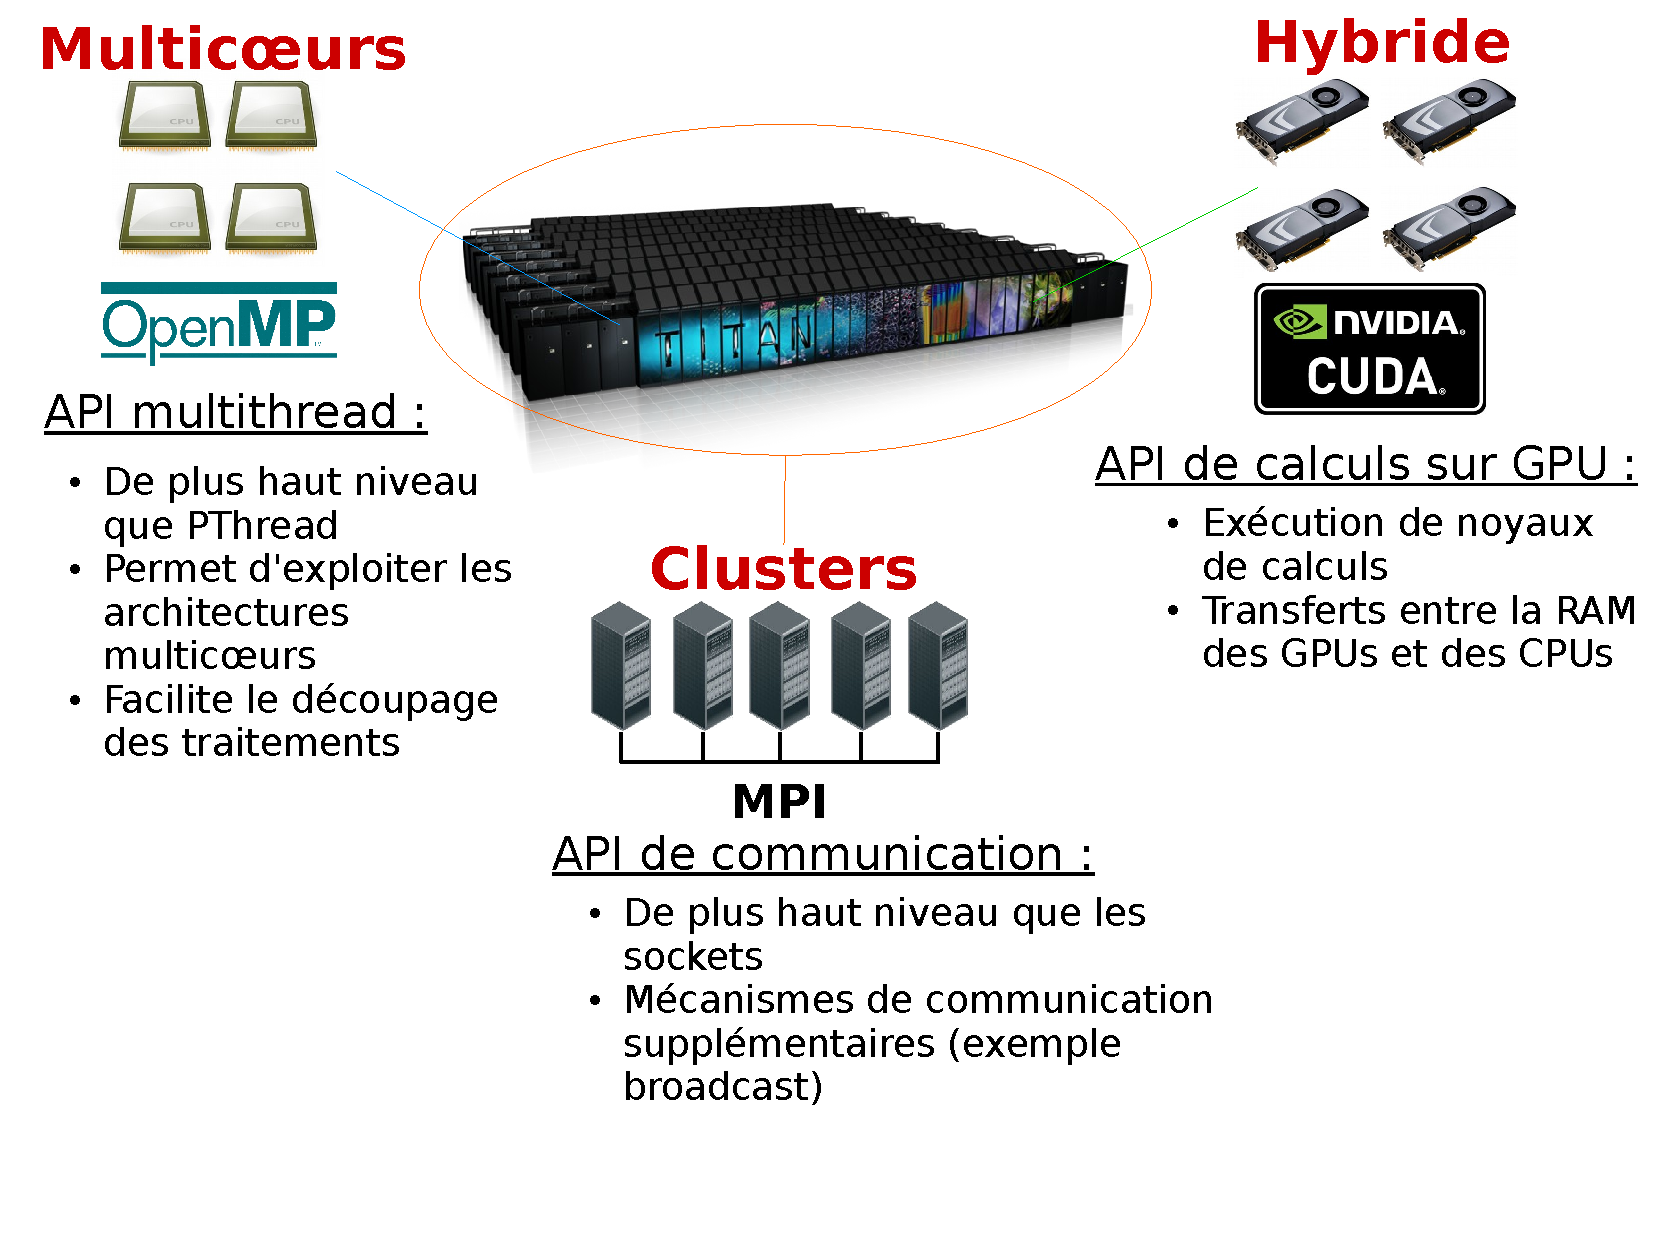
\includegraphics[width=\linewidth]{./Slides/Archi.pdf}
\end{figure}
\end{frame}

\begin{frame}[label=sec-1-2]{Limites des approches classiques}
\begin{itemize}
\item Utiliser \alert{plusieurs paradigmes} $\leadsto$ \alert{programmation complexe}
\item Exemple pour exploiter efficacement un GPU sur \alert{un seul noeud}:
\begin{itemize}
\item transférer données du CPU au GPU,
\item lancer le calcul sur le GPU
\item gérer synchronisation pendant attente résultat
\item occuper CPU
\item récupérer résultat.
\end{itemize}
\item Et avec \alert{plusieurs noeuds/cores/GPUs} ?
\begin{itemize}
\item \alert{Statique}, système réglé comme une horloge $\leadsto$ pas scalable.
\item Solution: Dynamique mais \alert{très difficile avec APIs classiques}.
\end{itemize}
\end{itemize}
\end{frame}
\begin{frame}[label=sec-1-3]{Nouvelle approche: paradigme de tâches}
\begin{columns}
  \begin{column}{.55\linewidth}
\begin{itemize}
\item Nouvelle abstraction: les tâches
\begin{itemize}
\item \alert{Plus besoin de se soucier de la ressource} sur laquelle le
traitement est effectué
\item Exprimer calcul en terme \alert{graphe de tâches} $\leadsto$ plus de
\alert{souplesse} et une meilleure \alert{portabilité}
\end{itemize}
\end{itemize}

  \end{column}
  \begin{column}{.35\linewidth}
    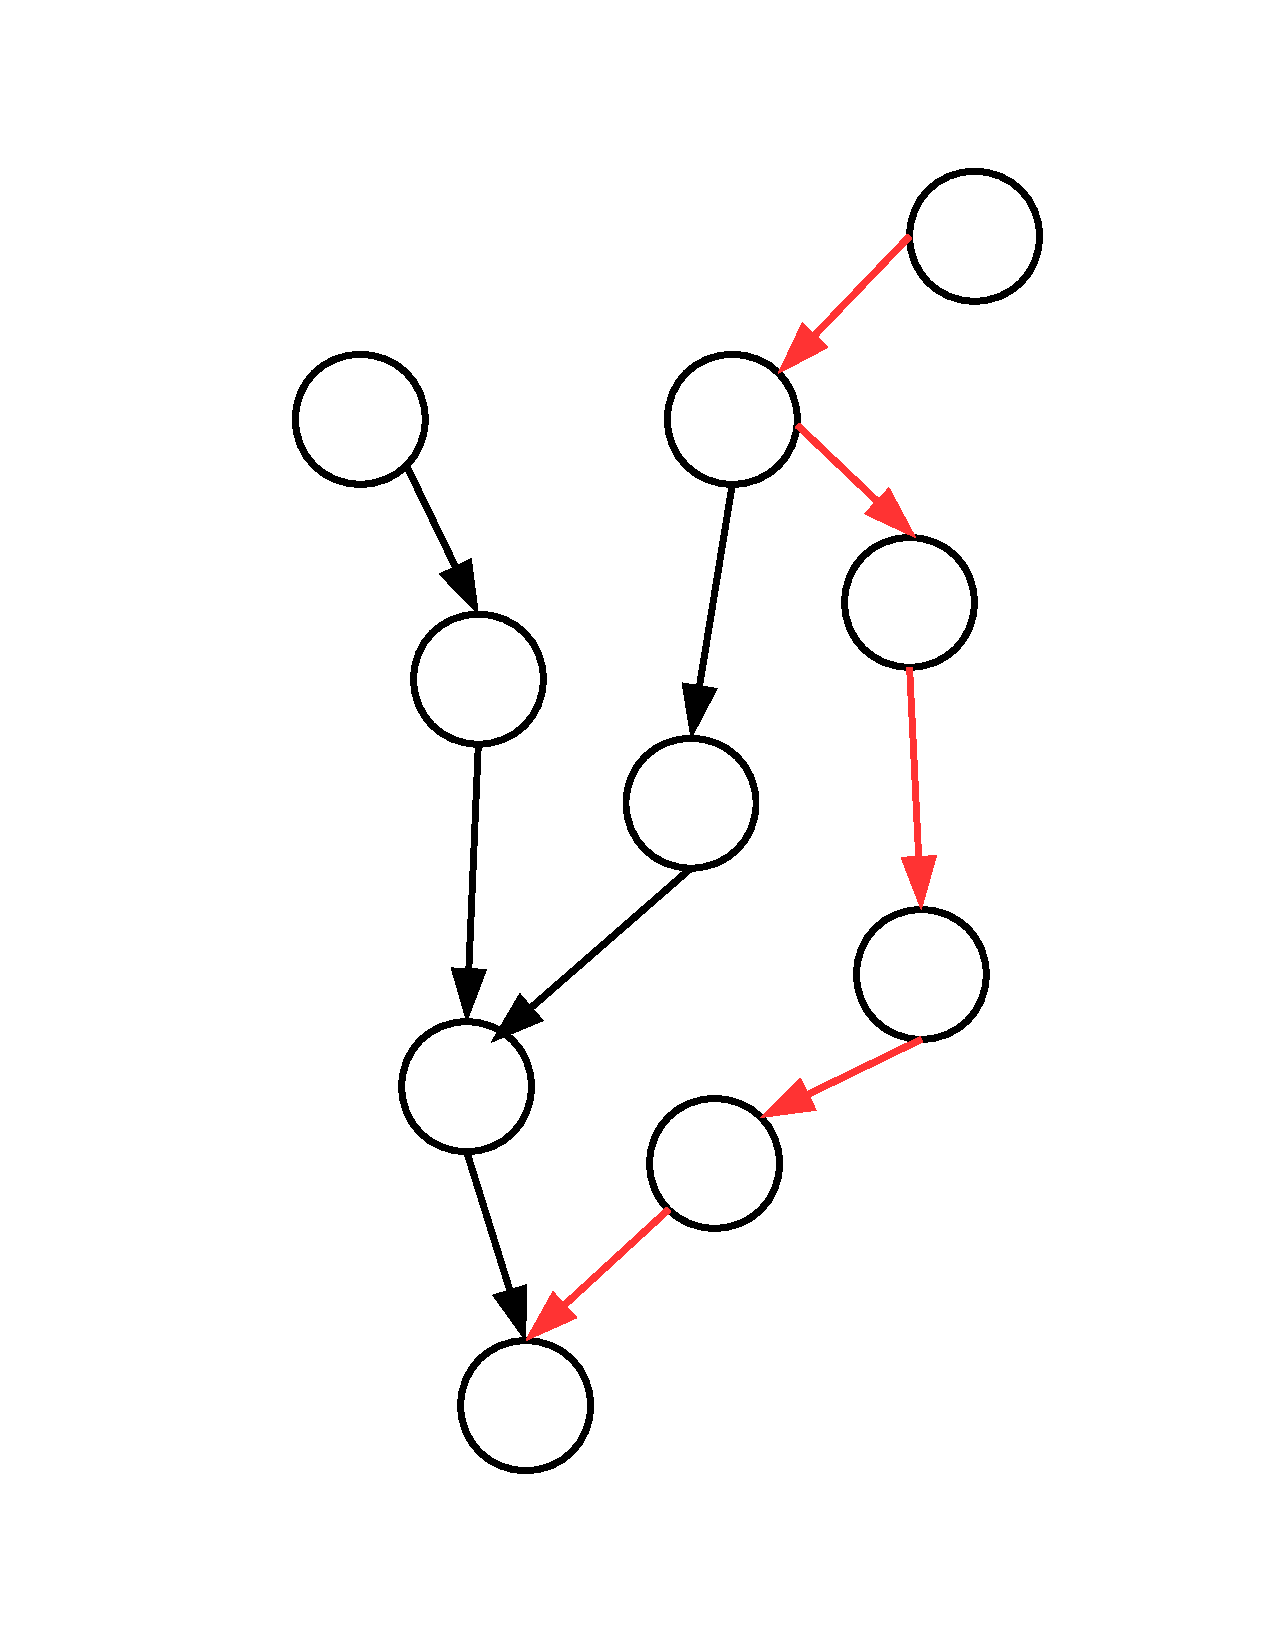
\includegraphics[width=.7\linewidth]{../Img/task_graph.pdf}%
  \end{column}
\end{columns}

\begin{itemize}
\item Librairie StarPU:
\begin{itemize}
\item Un runtime développé au LaBRI (RUNTIME/STORM).
\item Graphe de dépendances $\leadsto$ ordonnancemment \alert{dynamique et opportuniste}
\item Première version pour système hybrique et récémment StarPU MPI
\end{itemize}
\item \alert{Problèmatique} : Performances difficiles à évaluer car exécution du
flot de contrôle non déterministe
\begin{itemize}
\item Configuration \alert{runtime}, heuristique d'ordonnancement
\item Configuration \alert{application}, découpage en tâches
\end{itemize}
\end{itemize}
\end{frame}
\begin{frame}[label=sec-1-4]{Évaluation des performances en HPC: grandes approches}
\begin{block}{Test sur systèmes réels}
\begin{itemize}
\item Exécution réelle sur la plateforme cible $\leadsto$ \alert{coûteux,
difficulté d'accès}
\item Exécution \alert{non déterministe} nécessite de réaliser beaucoup
d'expériences $\leadsto$ extrapolations difficiles
\end{itemize}
\end{block}
\begin{block}{Simulation : Généralités}
\begin{itemize}
\item Utilisation de \alert{modèles} pour \alert{prédire} comportements
\item Permet \alert{s'affranchir de la plateforme} $\leadsto$ \alert{peu coûteux}
\item Extrapolation simplifiée / simulation très rapide
\end{itemize}
\end{block}
\end{frame}

\begin{frame}[label=sec-1-5]{Simulation: 2 possibilités}
\begin{block}{Simulation par rejeu de trace}
Pas adapté ici car \alert{flot de contrôle non déterministe}
\end{block}
\begin{block}{Hybride simulation / émulation}
\begin{itemize}
\item Simulation réaliste $\leadsto$ \alert{exécuter vrai code}
\item Simuler \alert{plate-forme et OS}.
\item Émuler de l'\alert{application}.
\end{itemize}
SimGrid simulateur de systèmes distribués, grilles de calculs,
systèmes peer to peer et cloud. 

StarPU SimGrid, approche simulation / émulation mais avec  \alert{un seul
noeud}. 
\end{block}
\end{frame}
\section{Analyse du problème}
\label{sec-2}
\begin{frame}[label=sec-2-1]{SimGrid: Généralités}
\begin{figure}
\centering
\vspace{-4.5mm}
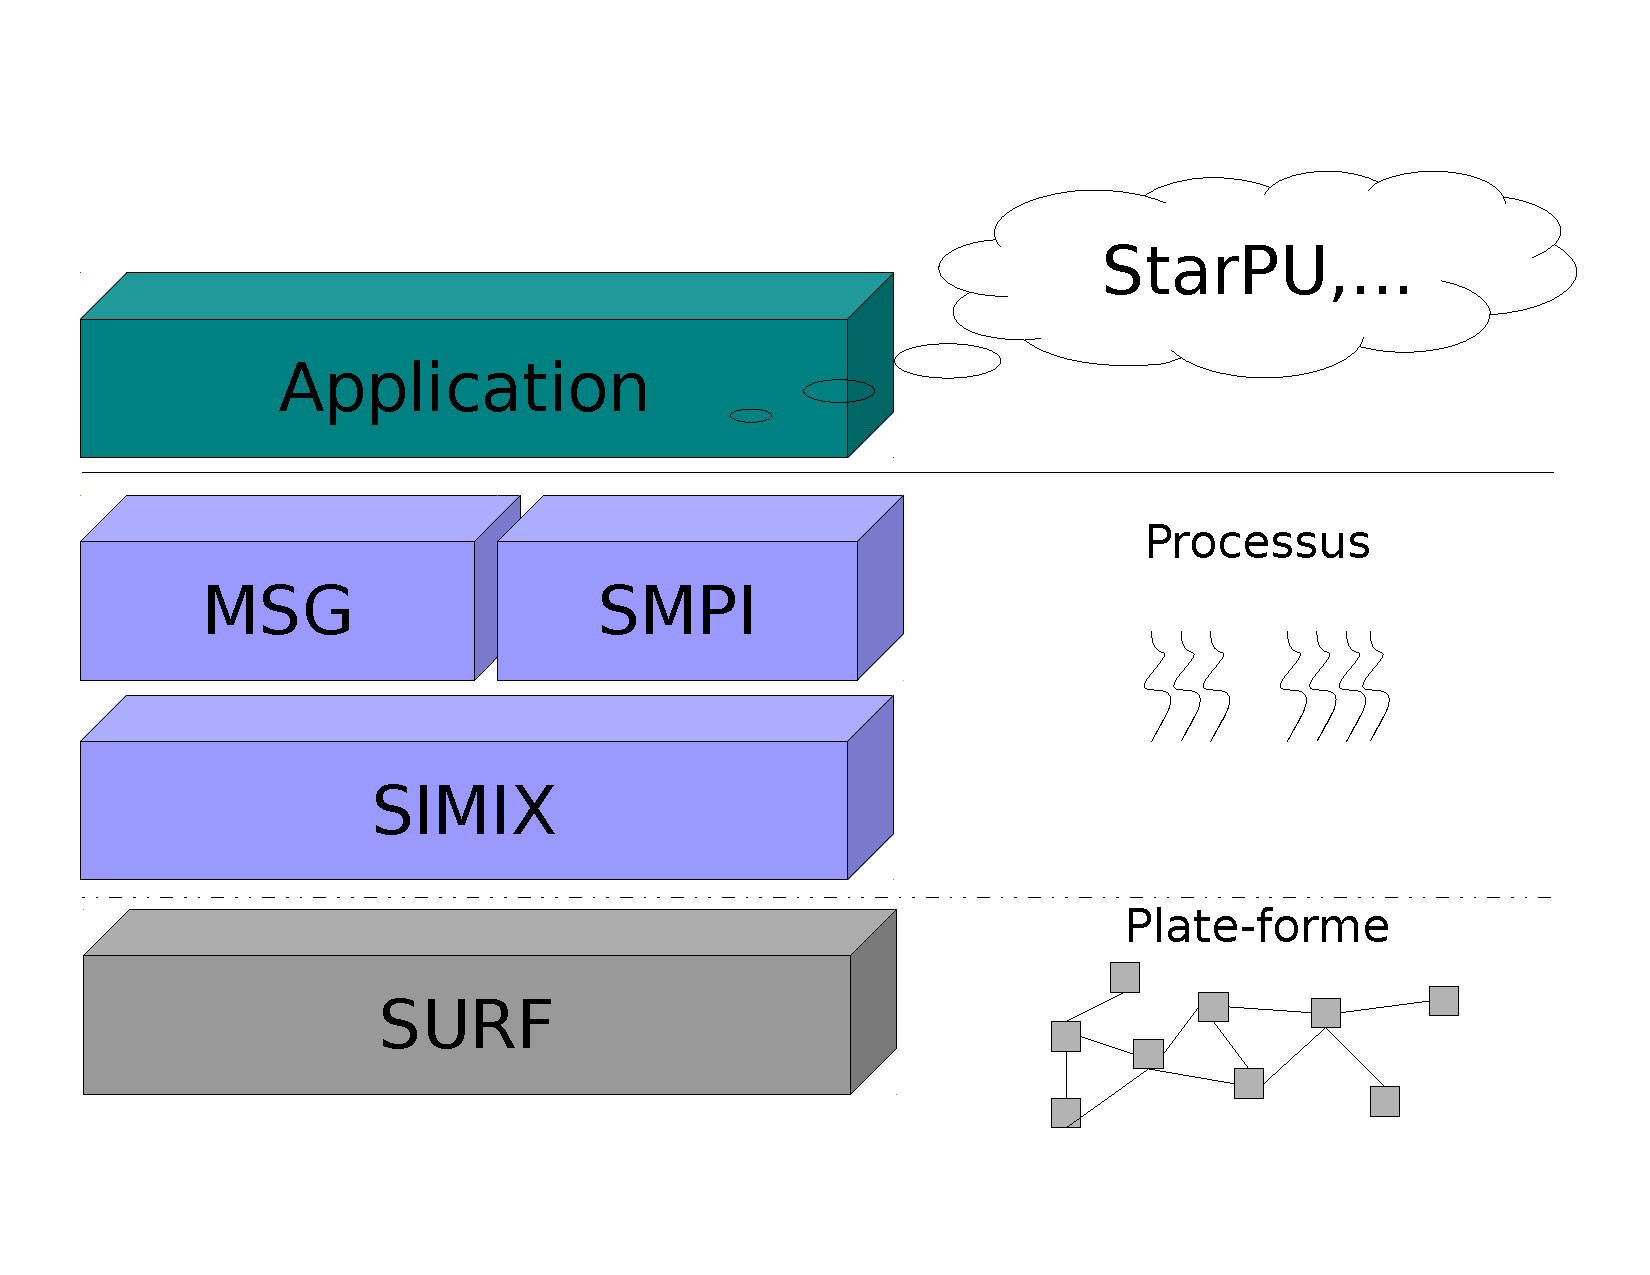
\includegraphics[width=\linewidth]{../Img/Simgrid.pdf}
\end{figure}
\end{frame}

\begin{frame}[label=sec-2-2]{Construction de l'application MPI simulée}
\begin{figure}
\centering
\vspace{-3.5mm}
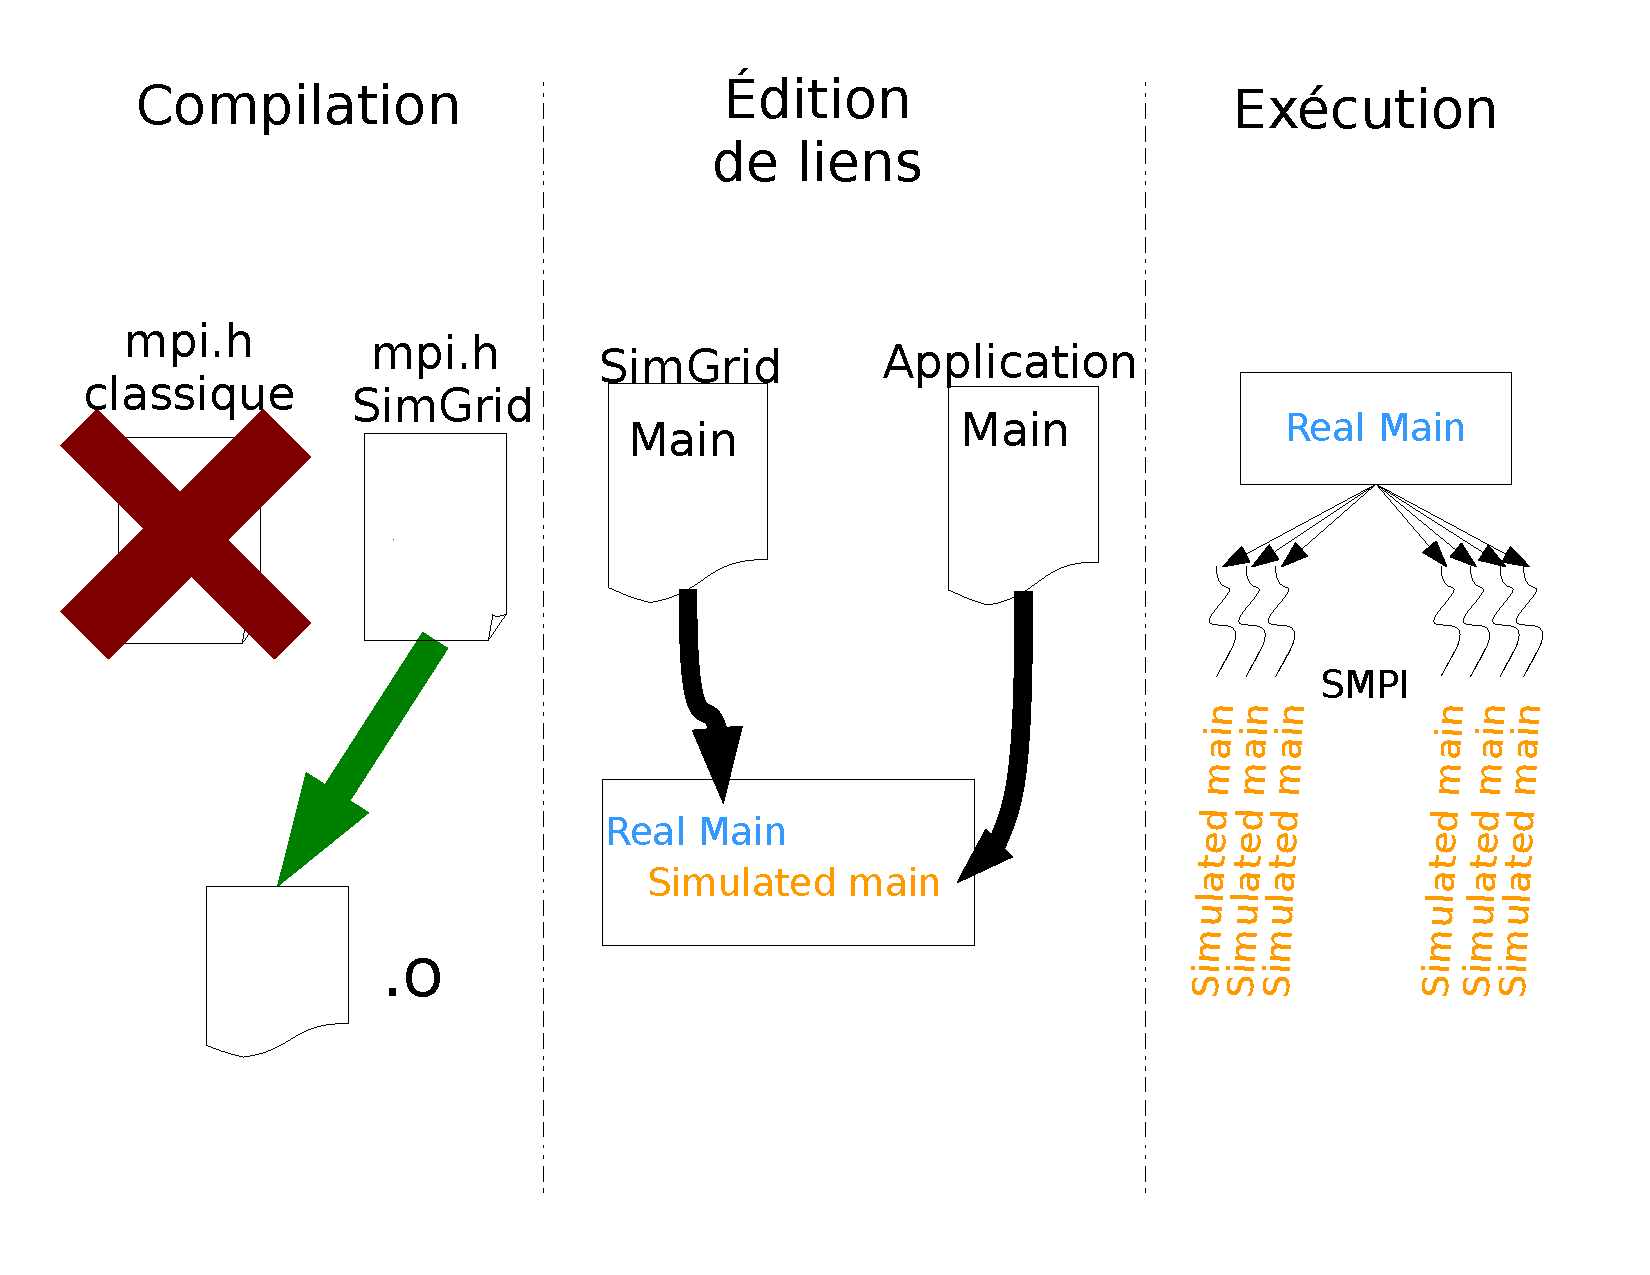
\includegraphics[width=\linewidth]{./Slides/Compilev2.pdf}
\end{figure}
\end{frame}
\begin{frame}[label=sec-2-3]{Privatisation du segment data}
\begin{columns}
  \begin{column}{.45\linewidth}
\begin{itemize}
\item Dans SimGrid les \alert{processus} sont \alert{modélisés par des threads} $\leadsto$
  espace adressage partagé.
\item MPI environnment à \alert{mémoire distribuée}.
\item Mécanisme de privatisation: \alert{ségment virtuel} (mmap)
\end{itemize}


  \end{column}
  \begin{column}{.45\linewidth}
    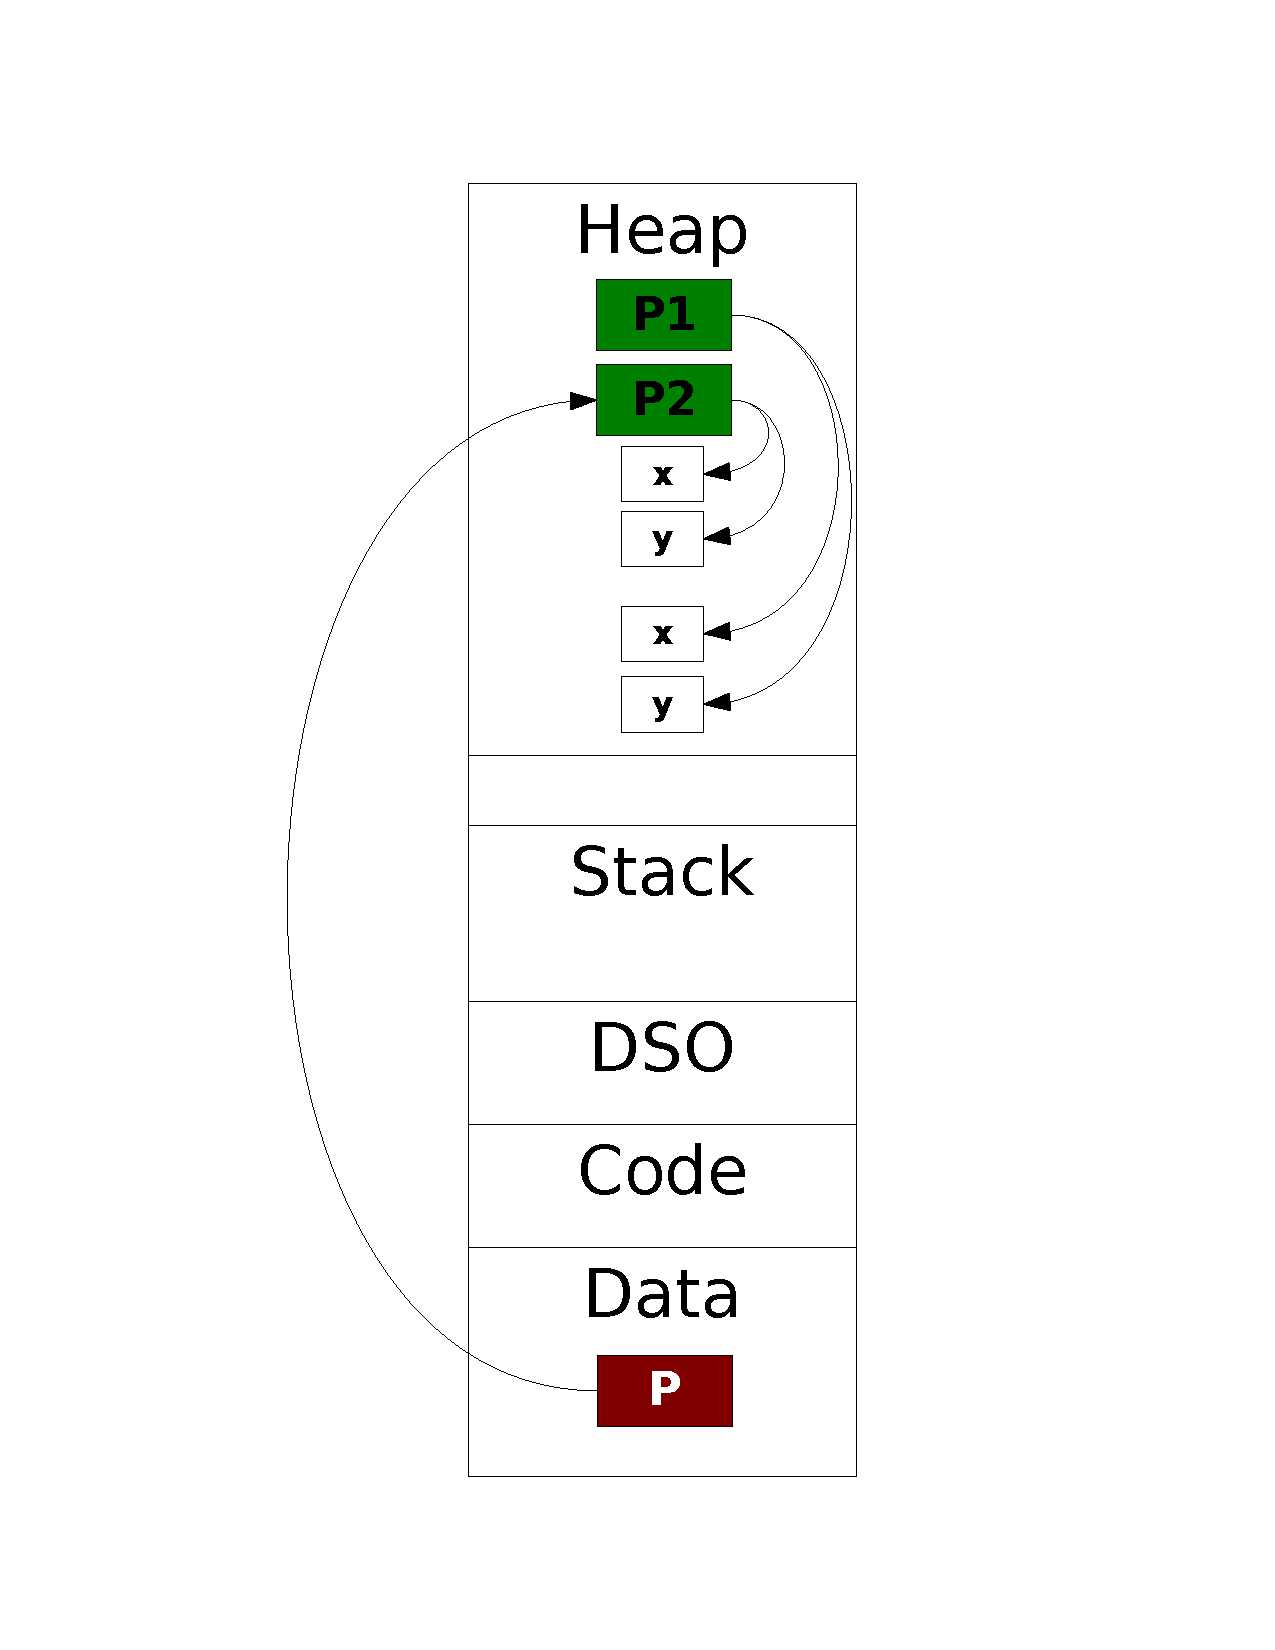
\includegraphics[width=\linewidth]{../Img/Memoire.pdf}
  \end{column}
\end{columns}
\end{frame}

\begin{frame}[label=sec-2-4]{StarPU MSG}
\begin{itemize}
\item Première version StarPU $\leadsto$ hybride
\item Basé sur \alert{MSG} car \alert{modèle de performance plus proche} (communications,
environnement mémoire partagé), CPUs GPUs.
\item Émulation: le vrai code de l'ordonnanceur de StarPU et de
l'application sont exécutés
\item Simulation: calculs, allocations mémoire des tâches, transfert
CUDA.

\begin{figure}
\centering
\vspace{-1.5mm}
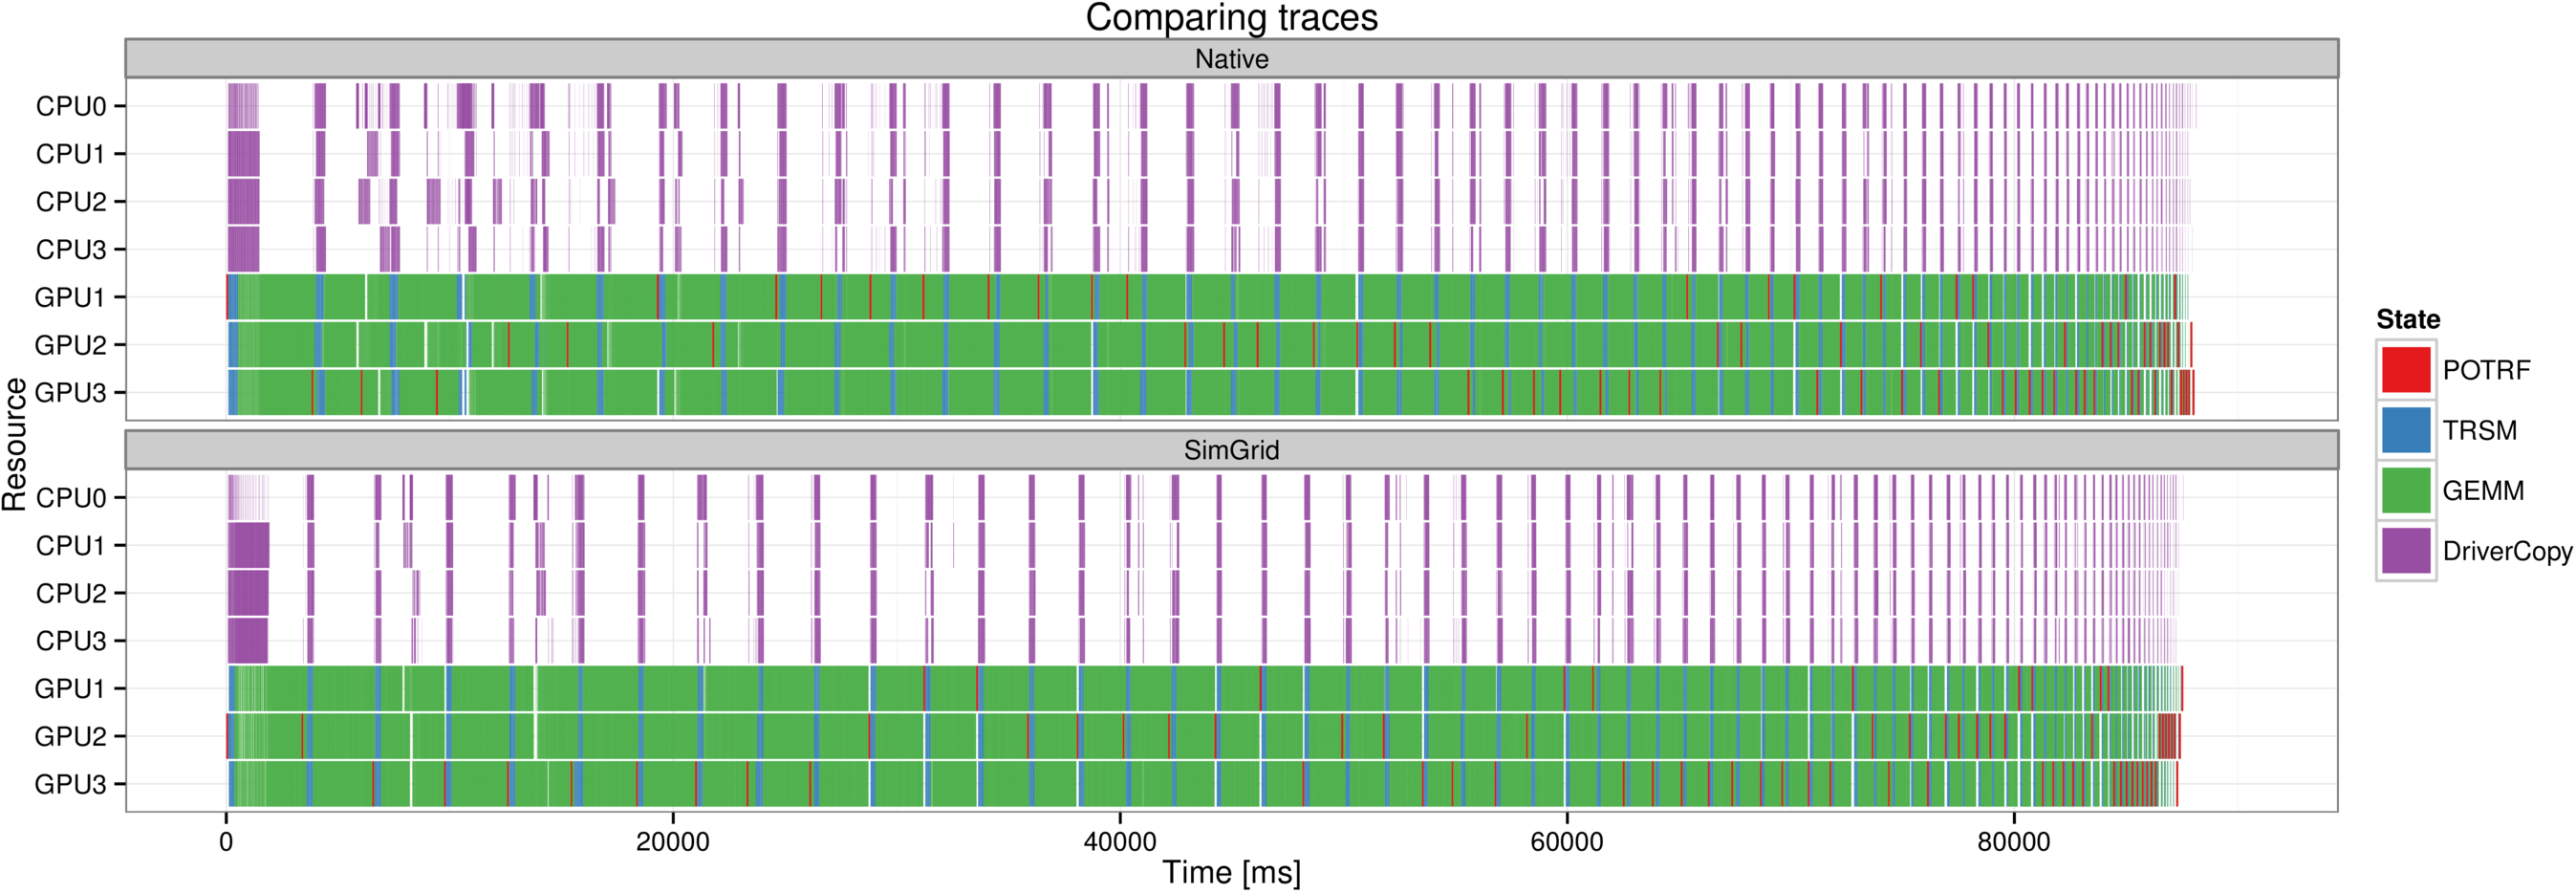
\includegraphics[width=\linewidth]{../Img/comparing_paje2-crop.png}
\end{figure}
\end{itemize}
\end{frame}

\begin{frame}[label=sec-2-5]{StarPU SMPI: Difficultés de mise en oeuvre}
\begin{itemize}
\item Besoin de 2 modèles de programmation différents à la fois:
\begin{itemize}
\item StarPU intra noeuds: mémoire partagée $\leadsto$ MSG, partage
\item StarPU inter noeuds: mémoire distribuée $\leadsto$ SMPI, privatisation
\end{itemize}

\item Besoin de 2 modèles de performance différents à la fois:
\begin{itemize}
\item StarPU intra noeuds: CPU-GPU $\leadsto$ MSG ad hoc
\item StarPU inter noeuds: réseau $\leadsto$ SMPI
\end{itemize}
Besoin de modifications un peu complexes dans SURF $\leadsto$ pas
dans le cadre de ce stage.
\item MSG et SMPI normalement pas utilisés ensemble $\leadsto$ initialiser
correctement les 2.
\end{itemize}
\vspace{-3.5mm}
  \begin{columns}[]
    \begin{column}{.55\linewidth}
\begin{itemize}
\item Problème des bibliothèques dynamiques.
\end{itemize}
  \end{column}
  \begin{column}{.35\linewidth}
 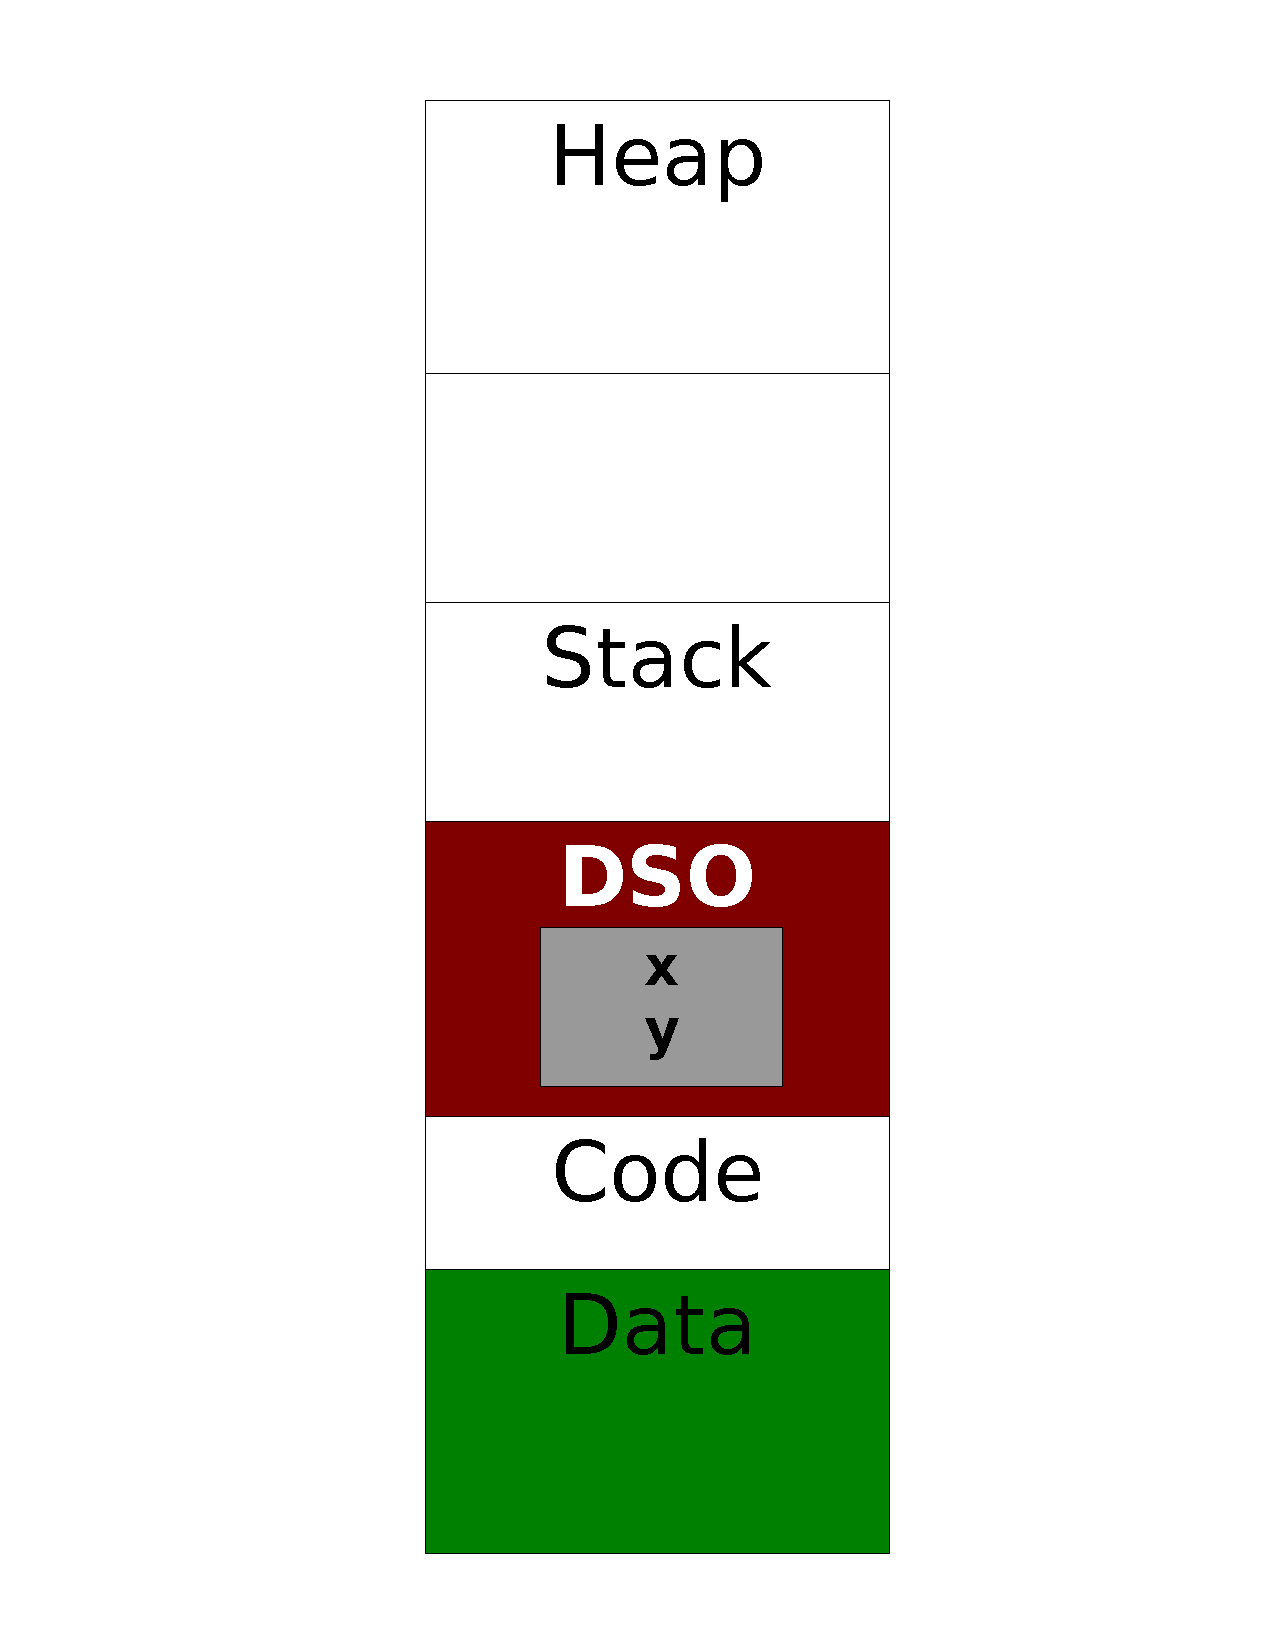
\includegraphics[width=.7\linewidth]{../Img/Dyn.pdf}
  \end{column}
\end{columns}
\end{frame}

\section{Méthodologie}
\label{sec-3}
\begin{frame}[label=sec-3-1]{Techniques et étude de l'existant}
\begin{block}{Prise en main}
\begin{itemize}
\item Dépôt git submobules:
\begin{itemize}
\item StarPU SMPI:
\begin{itemize}
\item SimGrid
\item StarPU
\end{itemize}
\end{itemize}
\item \alert{Suivi}:
\begin{itemize}
\item Cahier de laboratoire org mode github.
\end{itemize}
\item \alert{Compréhension}:
\begin{itemize}
\item Documentation.
\item SimgGrid = \alert{106 350 lignes} de codes.
\item StarPU = \alert{172 251 lignes} de codes.
\item "\alert{Code mining}" et vérifications: GDB, Valgrind.
\end{itemize}
\end{itemize}
\end{block}
\begin{block}{Validation}
\begin{itemize}
\item Test simple: Modèle simplifié de StarPU MPI $\leadsto$ isoler problèmes.
\item Test StarPU: MPI, Cholesky $\leadsto$ valider modifications
\end{itemize}
\end{block}
\end{frame}
\section{Contribution}
\label{sec-4}
\begin{frame}[label=sec-4-1]{Modification de SimGrid}
\begin{itemize}
\item Initialisation MSG + SMPI
\item Gestion du segment data: les processus MSG créés par un processus
SMPI "héritent" du segment de leur père.
\begin{figure}[tbh]
\centering
\vspace{-1.5mm}
   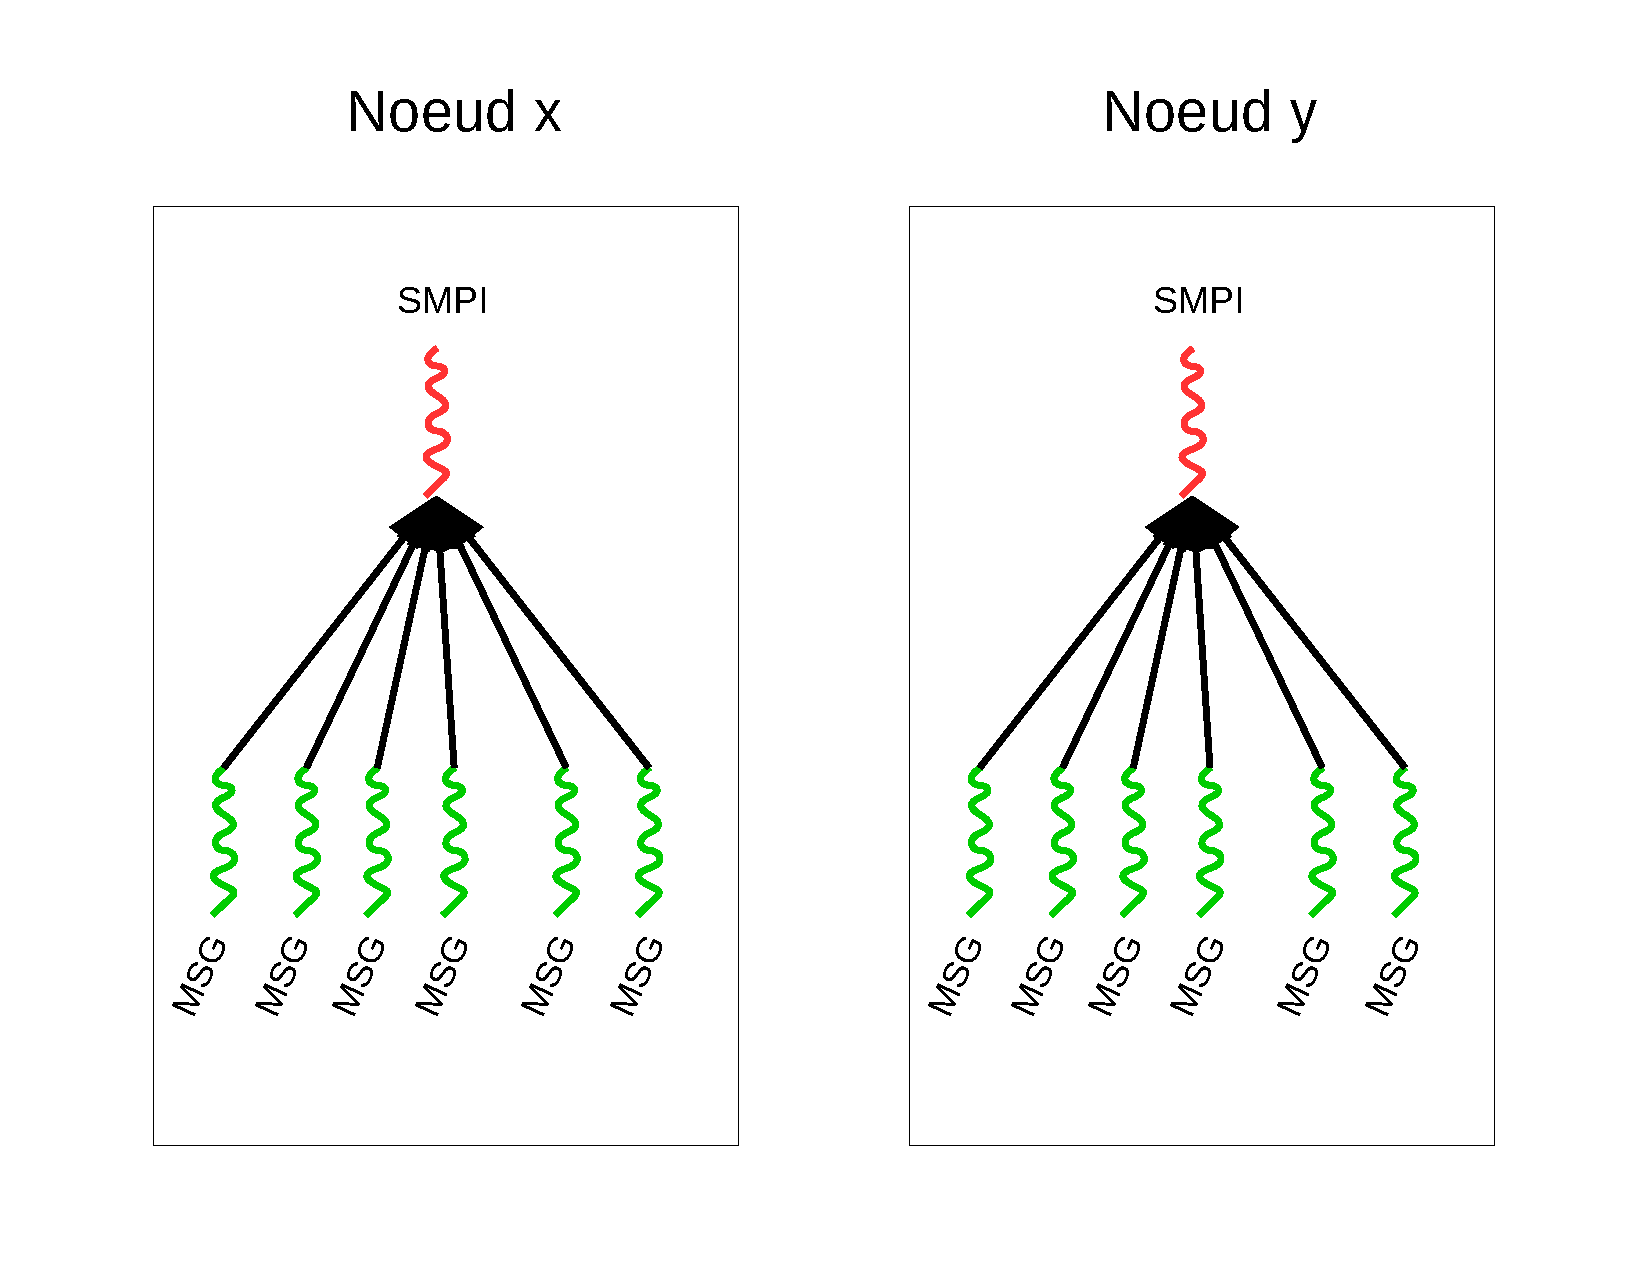
\includegraphics[height=.7\paperheight]{../Img/Processus.pdf}
\end{figure}
\end{itemize}
\end{frame}

\begin{frame}[label=sec-4-2]{Librairie dynamiques et modifications StarPU}
\begin{columns}
  \begin{column}{.6\linewidth}

\begin{itemize}
\item Librairies dynamiques:
\begin{itemize}
\item Utilisation librairies statiques.
\end{itemize}
\item Modification StarPU:
\begin{itemize}
\item Initialisation, car privatisation tardive.
\end{itemize}
\end{itemize}
  \end{column}
  \begin{column}{.35\linewidth}
    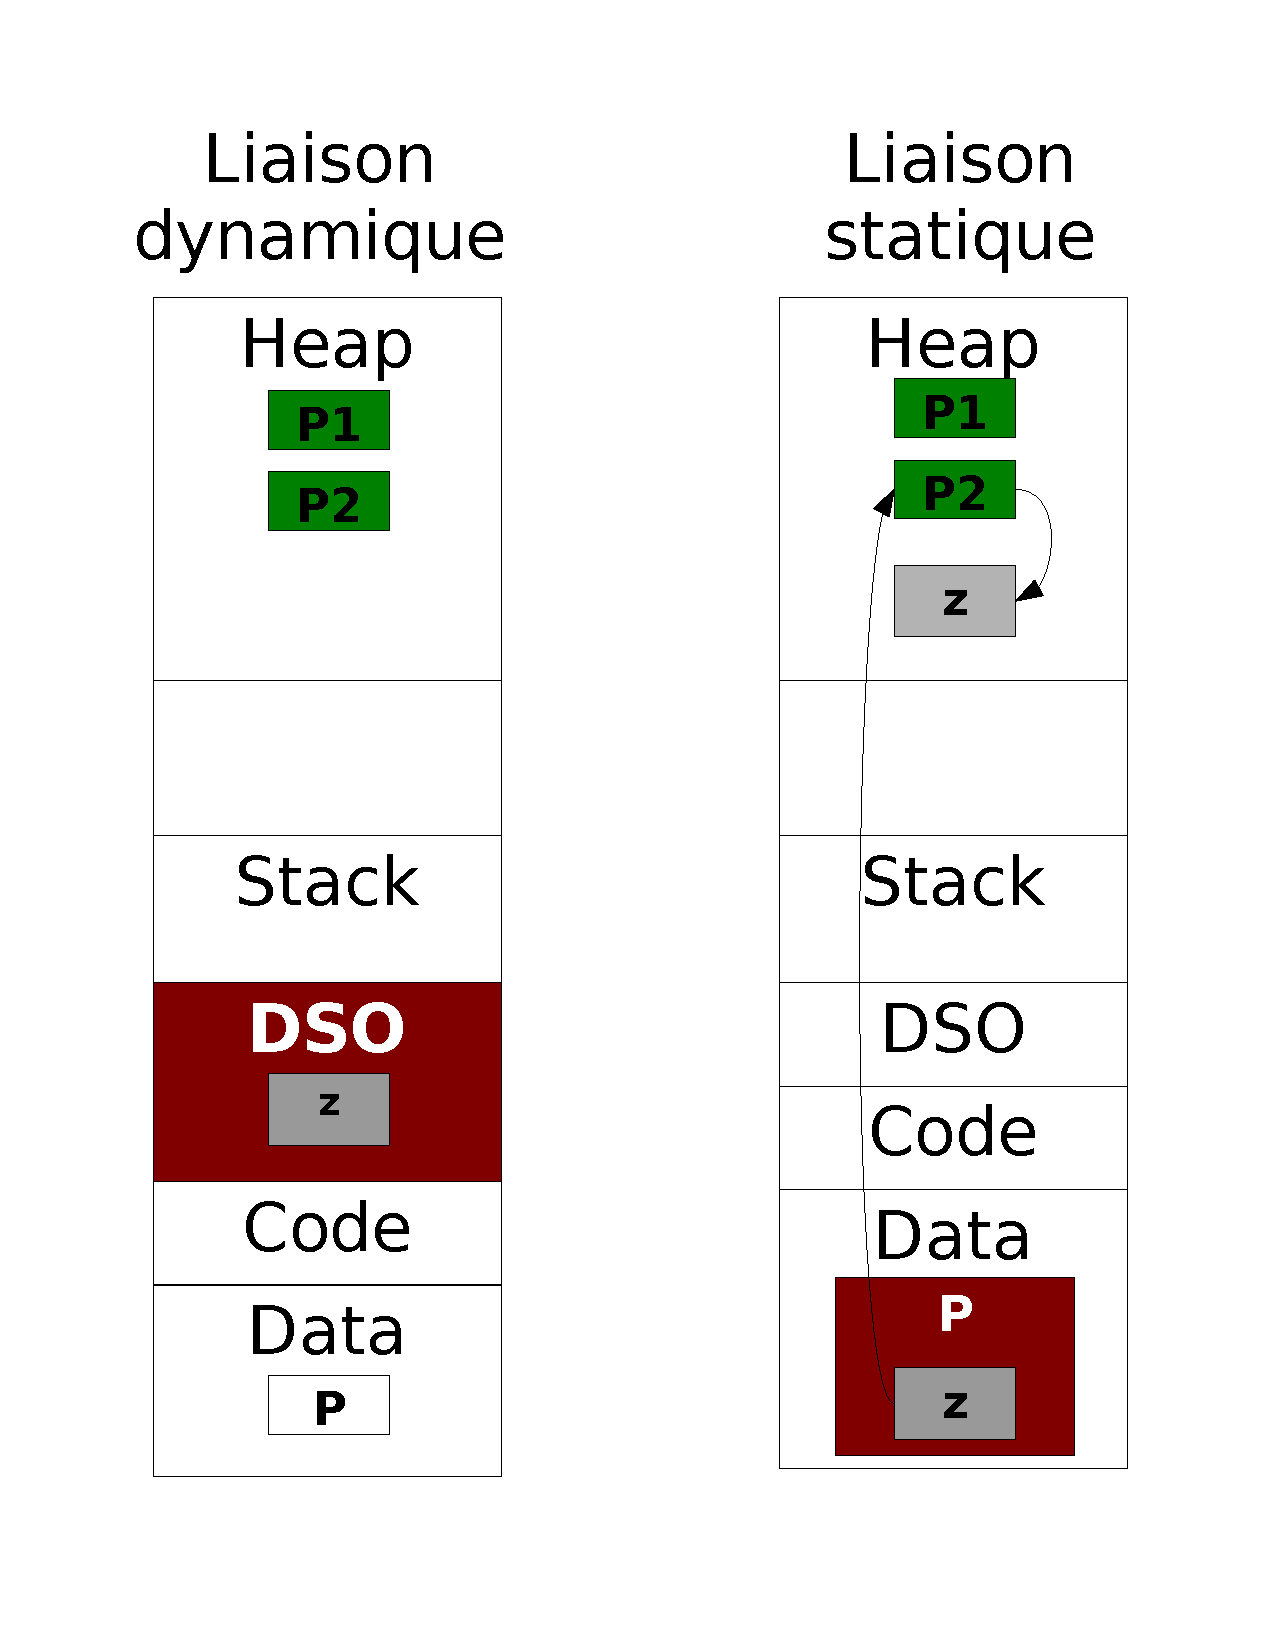
\includegraphics[width=\linewidth]{../Img/StaticDyn.pdf}
  \end{column}
\end{columns}
\end{frame}

\section{Conclusion}
\label{sec-5}
\begin{frame}[label=sec-5-1]{Pour conclure}
\begin{block}{Bilan}
\begin{itemize}
\item \alert{StarPU + SimGrid modifié} pour simuler StarPU MPI
\item Difficulté: apporter \alert{modifications minimes} dans un code \alert{non
trivial}. Environ 20 lignes sur un total de plus de 270 000
\end{itemize}
\end{block}
\begin{block}{Prochaine étape}
\begin{itemize}
\item \alert{Simulations et mesures} avec solveur d'algèbre linéaire
\item \alert{Vérifications système réel}: Grid5000
\item stabiliser le prototype (intégrer les modifications aux dépots
principaux de StarPU et de SimGrid)
\end{itemize}
\end{block}
\end{frame}

\begin{frame}[label=sec-5-2]{Rermerciements}
Merci pour votre attention.

Merci à Arnaud LEGRAND pour m'avoir permis de faire une stage dans son
équipe et pour avoir été autant disponible.
\end{frame}
% Emacs 24.5.1 (Org mode 8.2.10)
\end{document}